
\section{Armado del dispositivo}
Un supercondensadores es armado simplemente haciendo un sandwich electrodo-separador-electrodo, siendo los electrodos con material el componente más crítico. Los electrodos son placas metálicas que cumplen el rol de colectores de corriente, recubiertos con el materiales que se desea utilizar, en este caso, RGO.\circled{1}

\begin{figure}[h!]
	\centering
	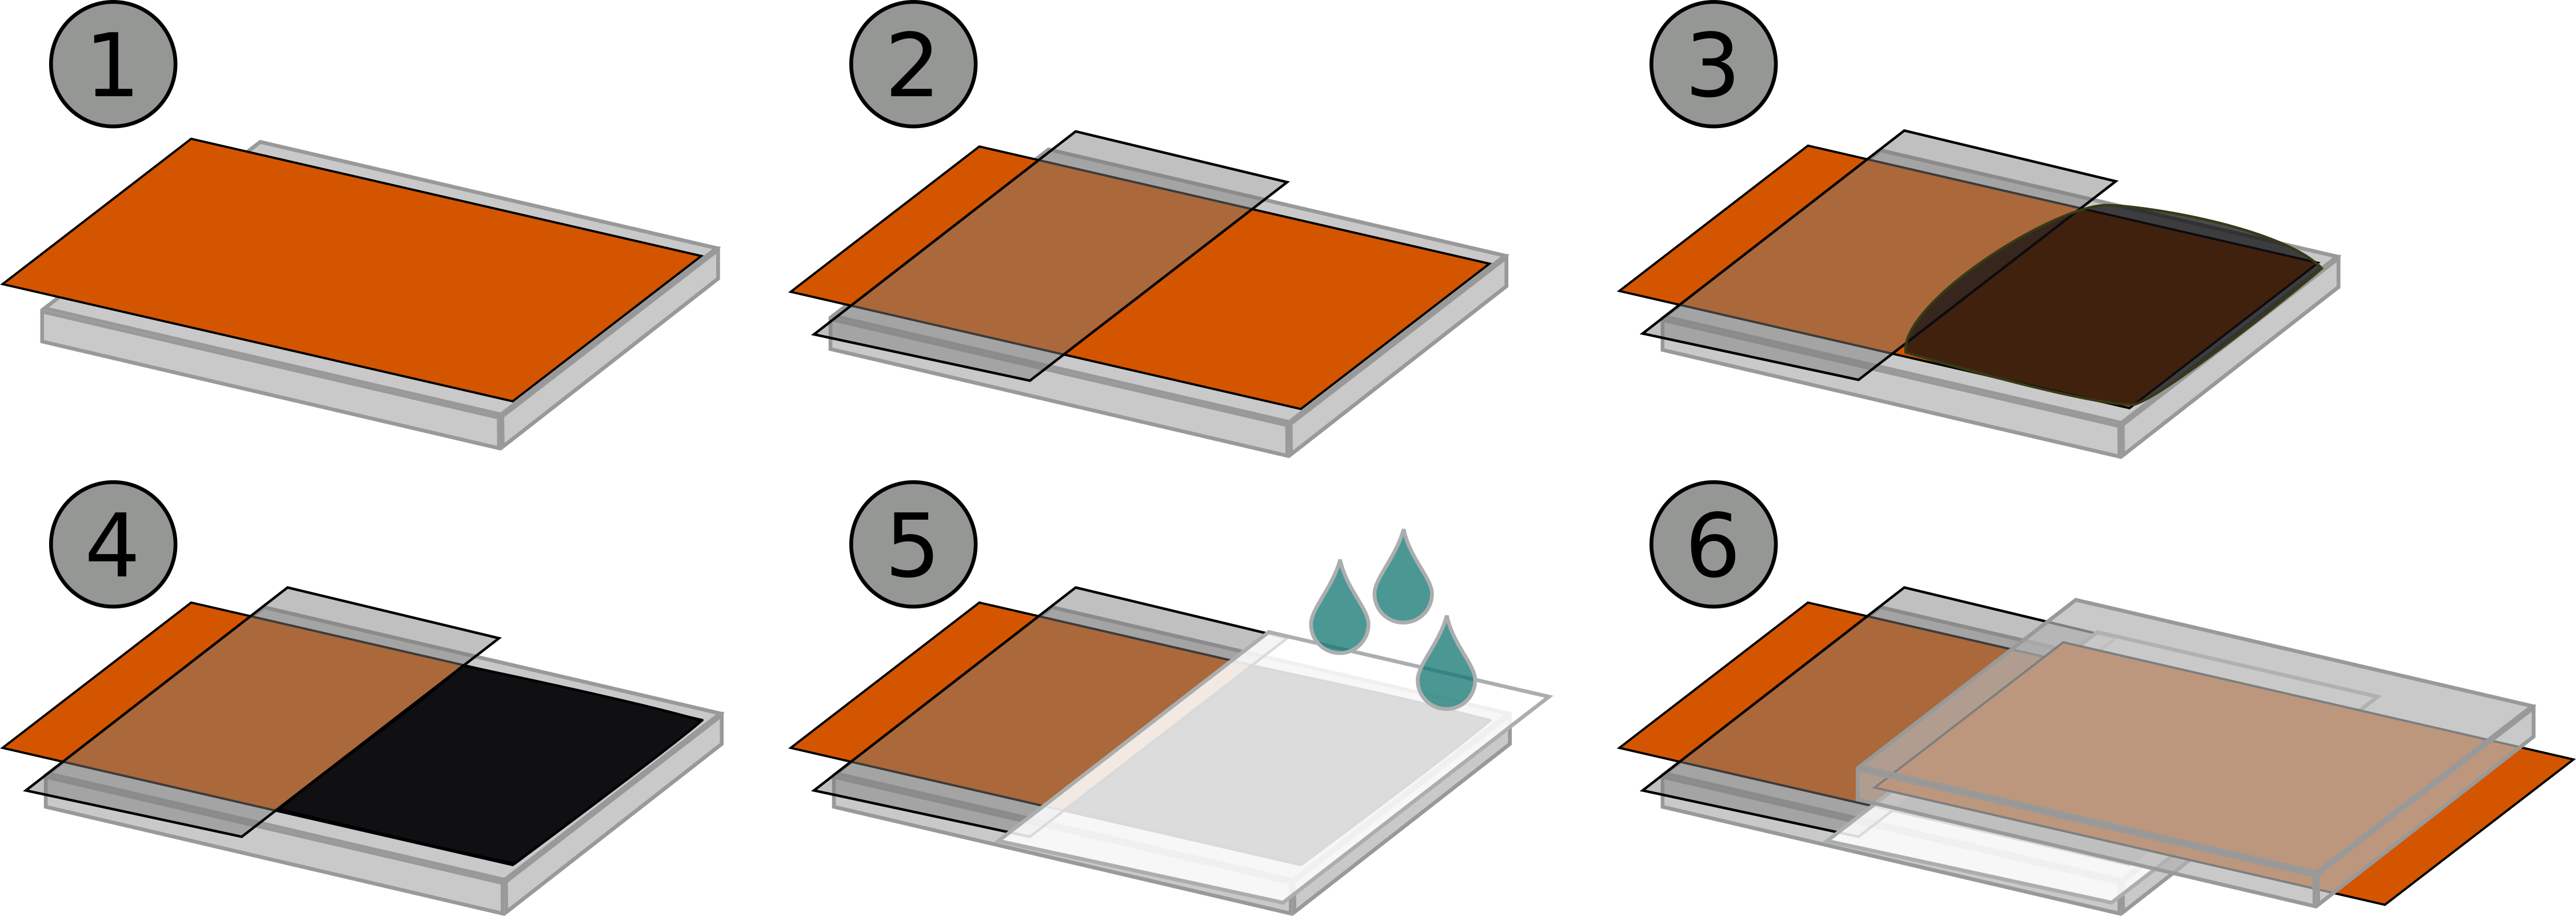
\includegraphics[width=1\textwidth]{SC_process.png}
	\label{fig:SC_process}
	\caption{Armado de un supercondensador para realizar pruebas.\protect\circled{\small 1}Lámina metálica de 1 cm de ancho sobre un trozo de vidio. \protect\circled{2} Cinta auto adhesiva para limitar el área a 1 cm\protect\textsuperscript{2}.}
\end{figure}
\section{Celda de prueba de supercondensador}

\begin{figure}[h!]
	\centering
	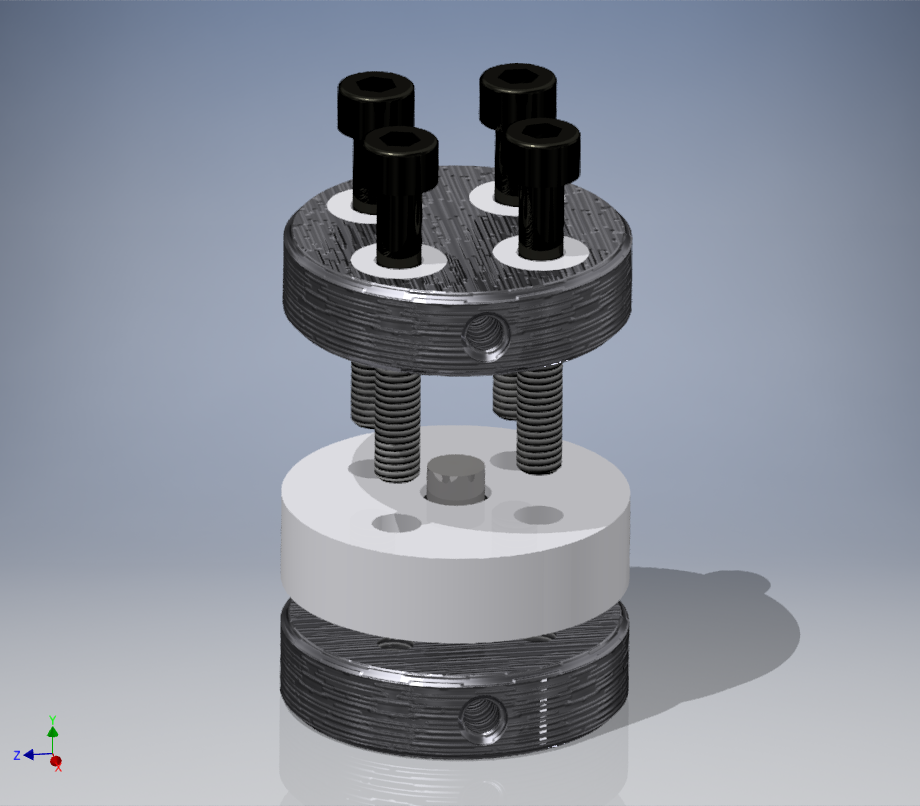
\includegraphics[width=0.5\textwidth]{cell4.png}
	\label{fig:celda_de_pruebas_SC}
\end{figure}


\section{Resultados}
Los supercondensadores son sometidos a pruebas electroquímicas estudiar su desempeño, estás pruebas incluyen: voltametría cíclica (CV), ciclos de carga y descarga a corriente constante, espectroscopía de impedancia electroquímica (EIS).
